\documentclass[UTF8,a4paper,10pt,fontset=fandol]{ctexart}
\usepackage[margin=17mm,headheight=12pt,headsep=6mm,footskip=9mm]{geometry}
\usepackage{amsmath,amssymb,booktabs,graphicx,xcolor,fancyhdr,enumitem,hyperref}
\definecolor{ink}{HTML}{183B37}\definecolor{accent}{HTML}{216B62}\definecolor{muted}{HTML}{62736C}
\hypersetup{colorlinks=true,urlcolor=accent,linkcolor=accent,pdftitle={梁鉴：环境扰动下的损伤识别},pdfauthor={}}
\pagestyle{fancy}\fancyhf{}\fancyhead[L]{\small\color{muted}AIC 2026\quad AI+力学 / 开放式赛题}\fancyhead[R]{\small\color{muted}技术报告}\fancyfoot[C]{\small\thepage}
\ctexset{section={format=\large\bfseries\color{ink},beforeskip=9pt,afterskip=5pt}}
\setlength{\parindent}{2em}\setlength{\parskip}{2pt}\linespread{1.08}
\newcommand{\HybridMAE}{0.135}
\newcommand{\PhysicsMAE}{0.150}
\newcommand{\AIMAE}{0.757}
\newcommand{\HybridTime}{21.6}
\newcommand{\PhysicsTime}{81.7}
\newcommand{\AITime}{3.9}
\newcommand{\Speedup}{3.78}
\newcommand{\CallSaving}{80.2}
\newcommand{\Coverage}{87.5}
\newcommand{\Width}{2.08}
\newcommand{\Accept}{97.5}
\newcommand{\HealthyFalseAblation}{44.2}
\newcommand{\MeshMAE}{0.128}
\newcommand{\TripleMAE}{4.77}
\newcommand{\MassMAE}{5.51}
\newcommand{\NoiseMAE}{0.801}
\newcommand{\FullSeconds}{128.8}
\newcommand{\HybridDamagedMAE}{0.517}

\begin{document}
{\noindent\color{accent}\small 固体力学 / 动力学与控制\hfill 团队编号：待补}\par
\vspace{6pt}{\noindent\fontsize{23}{29}\selectfont\bfseries\color{ink}梁鉴：环境扰动下的损伤识别}\par
\vspace{3pt}{\noindent\color{muted}AI候选筛选、物理反演与留出模态校核\hfill 2026年10月13日}
\section{作品概述}
梁结构的频率下降既可能来自局部损伤，也可能来自环境引起的整体刚度变化。梁鉴面向教学与试验梁，把整体刚度因子与局部刚度折减分别建模：随机树先筛选损伤位置，有限元反演估计损伤程度，第4、5阶模态检查结果的一致性。作品提供本地交互演示、逐例数据与复现程序。

\textbf{验证结论：}在120个常规域独立仿真样本上，六分区平均损伤误差为\HybridMAE 个百分点，定位完全匹配率100\%；推理中位耗时\HybridTime\,ms，穷举基线为\PhysicsTime\,ms。上述结论限于预设模型与噪声范围，尚无实物试验或现场应用证据。
\section{需求分析}
文献已指出环境变化会干扰振动损伤监测\cite{peeters}。本项目将需求限定为：在已知健康梁参数、已识别模态和少数局部损伤的条件下，降低位置搜索开销，同时保留可解释的反演过程与拒判依据。需求来源为文献研究和模型分析，未开展用户访谈。重点解决环境混淆、纯AI回归偏差及模型失配时过度确信三个问题。
\section{AI技术工具选择与运用}
采用本地Extra Trees回归器：每种子2400个训练样本、160棵树、叶节点最少2样本。输入为前三阶对数频率比与六点振型，输出六区损伤及整体刚度因子；取评分最高的三个位置，组成0、1、2处损伤共7个候选。选择随机树是因为样本规模小、CPU可训练、无需预训练模型；树算法与优化器使用公开库，非本项目原创。
\begin{center}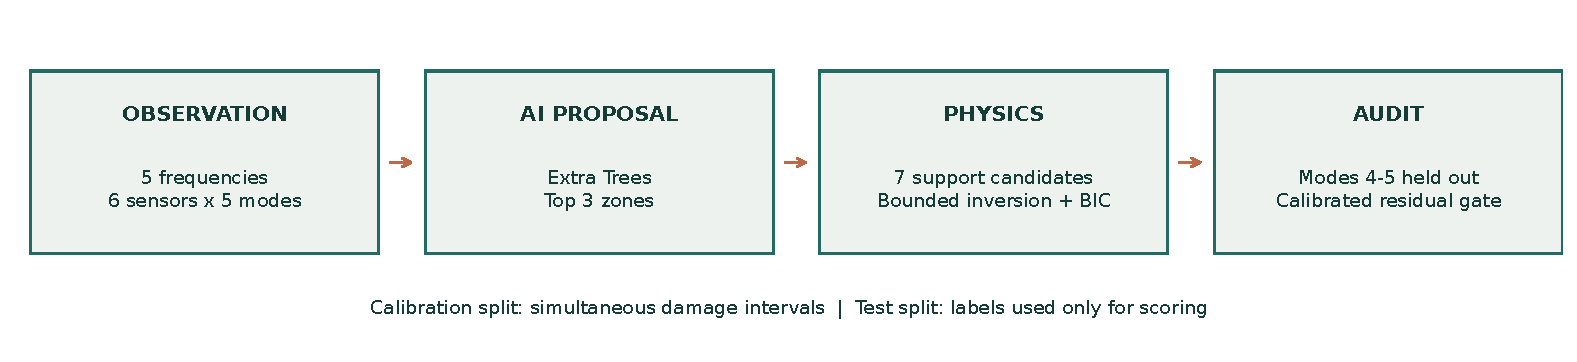
\includegraphics[width=\linewidth]{generated/workflow.pdf}\end{center}
\section{项目实施与关键技术}
均匀铝梁长1.2\,m、截面30\,mm$\times$6\,mm，$E=70$\,GPa、$\rho=2700$\,kg/m$^3$；划分6个损伤区、12个Euler--Bernoulli单元。由
\vspace{-3pt}
\begin{equation*}
K(\mathbf d,\alpha)=\alpha\sum_{j=1}^{6}(1-d_j)K_j^0,\qquad K\phi_r=\omega_r^2M\phi_r
\end{equation*}
建立模态到损伤的约束。对候选支持集$S$，求解加权残差最小化，并用复杂度惩罚选择支持集：
\vspace{-3pt}
\begin{equation*}
\min_{\substack{0\le d_j\le0.65,\;j\in S\\0.65\le\alpha\le1.35}}
\sum_{i\in\mathcal I}\left(\frac{g_i(\mathbf d,\alpha)-y_i}{\sigma_i}\right)^2,
\quad \mathrm{score}(S)=\mathrm{RSS}_S+(|S|+1)\ln21.
\end{equation*}
这是采用已知名义噪声尺度的BIC型选择准则。$d,\alpha$及频率比、归一化振型均无量纲；$\omega$单位为s$^{-1}$。工程贡献在于候选缩减、环境分离与校核的联动，不宣称发明基础算法。单次实验链包括训练、独立校准、六域测试和完整留痕，后续由团队复核、试验和答辩。
\newpage
\section{应用成效与实验校核}
使用3个独立种子；每种子2400训练、120校准、6域各40测试，总计720个独立测试样本、4种方法共2880条预测。所有数据均由本项目力学模型生成；训练、校准、测试使用不同随机流。与穷举全部22个候选的非线性反演使用相同物理目标、每候选35次迭代预算和相同观测。
\begin{center}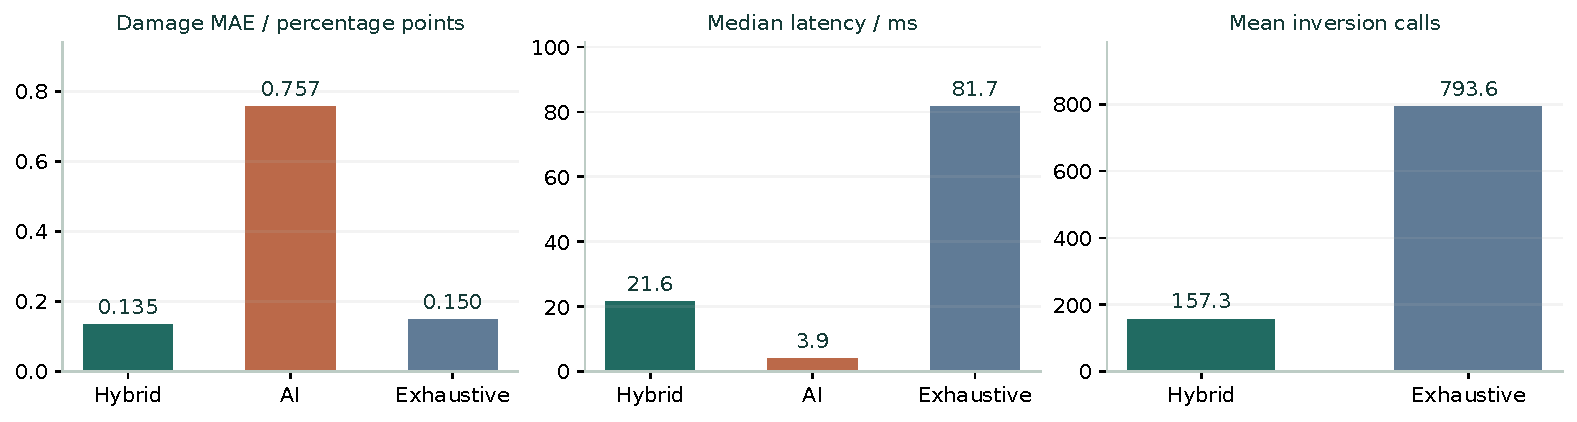
\includegraphics[width=\linewidth]{generated/headline.pdf}\end{center}
\vspace{-7pt}
\begin{center}\small
\begin{tabular}{lrrrr}\toprule
常规域方法 & 全区MAE/百分点 & 受损区MAE/百分点 & 定位F1 & 中位耗时/ms\\\midrule
AI+力学校核 & 0.135 & 0.517 & 1.000 & 21.6 \\
纯AI & 0.757 & 2.639 & 0.992 & 3.9 \\
穷举物理反演 & 0.150 & 0.524 & 1.000 & 81.7 \\
不估计环境（消融） & 3.248 & 10.644 & 0.667 & 53.5 \\
\bottomrule\end{tabular}

\end{center}
融合方案在本轮常规域的误差与穷举基线接近，耗时约为后者的$1/\Speedup$，前向调用减少\CallSaving\%。计时为同机单CPU线程在线推理，不含离线训练；整套3种子训练、校准和评估共\FullSeconds\,s。纯AI更快但误差较大，不将其回归结果直接当作物理诊断。健康环境变化组中，忽略环境因子的消融误报率为\HealthyFalseAblation\%，融合方案为0/120；零次误报不等于总体误报概率为零。

\textbf{不确定性与失败案例。}以独立校准集的最大分区误差构造90\%同时区间\cite{cp}，常规域实测覆盖率为\Coverage\%，平均宽度\Width 个百分点；没有将名义90\%写成实际达标。留出模态阈值取校准残差的95\%有限样本分位数。常规域接受率\Accept\%；三倍噪声、三处损伤、附加质量这三组各120例全部触发复核，但这不证明对任意未知异常均有效。
\begin{center}\small
\begin{tabular}{lrrrr}\toprule
测试域（各120例） & MAE/百分点 & 定位完全匹配/\% & 区间覆盖/\% & 校核接受/\%\\\midrule
常规域 & 0.135 & 100.0 & 87.5 & 97.5 \\
健康环境变化 & 0.082 & 100.0 & 90.8 & 97.5 \\
三倍噪声 & 0.801 & 79.2 & 28.3 & 0.0 \\
加密网格 & 0.128 & 100.0 & 90.8 & 95.0 \\
三处损伤 & 4.771 & 0.0 & 0.0 & 0.0 \\
附加质量 & 5.510 & 14.2 & 0.0 & 0.0 \\
\bottomrule\end{tabular}

\end{center}
\textbf{可复现性。}10项独立力学/数值测试通过；两次从头生成数据、训练模型并执行全域评估，全部非计时逐例结果、数据数组与校准记录一致。加密网格生成、粗网格识别的误差为\MeshMAE 个百分点，不能替代不同梁型或实测数据的泛化证明。
\section{总结与展望}
作品已形成从模态输入到诊断、区间与校核的本地闭环，适合力学教学和算法对照研究。当前仅适用于最多两处局部刚度损失；均匀损伤与整体刚度变化不可辨识。理想模态特征上的合成噪声未覆盖原始波形的模态识别误差、夹持松动和质量变化。下一步按预留工况开展实物梁试验，再评估传感器质量、温度与边界条件影响；未量化经济收益。

\vspace{2pt}{\noindent\small\textbf{附录材料：}《技术补充》含推导、全域结果与复现说明；代码包保留模型、原始样本、逐例记录和AI辅助声明。团队编号及参赛者人工审核待补。}
\vspace{-5pt}
\begin{thebibliography}{9}\small\setlength{\itemsep}{0pt}
\bibitem{peeters} Peeters B, Maeck J, De Roeck G. Vibration-based damage detection in civil engineering: excitation sources and temperature effects. Smart Materials and Structures, 2001, 10: 518--527. doi:10.1088/0964-1726/10/3/314.
\bibitem{cp} Angelopoulos A N, Bates S. A Gentle Introduction to Conformal Prediction and Distribution-Free Uncertainty Quantification. arXiv:2107.07511, 2021.
\end{thebibliography}
\end{document}
